\documentclass[10pt, conference, compsocconf]{IEEEtran}
\usepackage{graphicx}
\usepackage{float}
\usepackage{amsmath}
\usepackage{hyperref}
\usepackage{multirow}
\usepackage{array}

\hypersetup{
	colorlinks=true,
	linkcolor=black,
	filecolor=magenta,      
	urlcolor=cyan,
}



\title{Fuzzy inference system}

\begin{document}
	
	\maketitle
	
	
	\section{Model}
	\begin{figure}[h!]
		\centering
		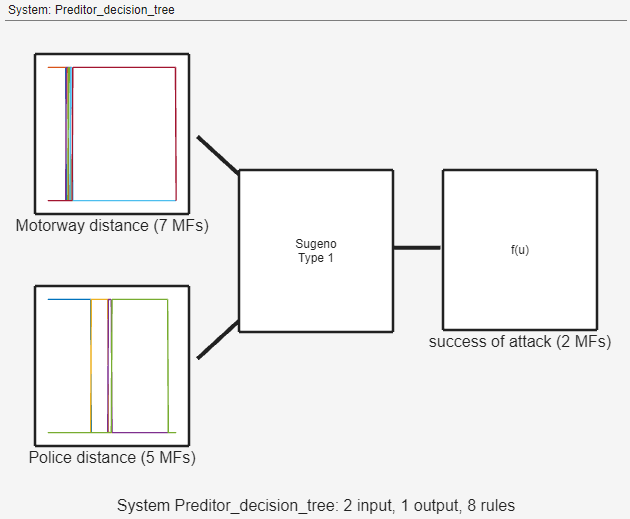
\includegraphics[width=\linewidth]{Fuzzy_1.png}
		\caption{Fuzzy inference System}
		\label{fis}
	\end{figure}

    \textbf{Model specification}
    \begin{enumerate}
    	\item Model type: Sugeno Type-1 \href{https://in.mathworks.com/help/fuzzy/types-of-fuzzy-inference-systems.html}{(Matlab referece)}
    	\item likelihood function: Fuzzy maximum likelihood estimation
    	\item Input(Antecedent): Police distance \& Motorway distance
    	\item Output(Consequent): Success of attack
    \end{enumerate}
	\vspace{5pt}
	In Figure \ref{fis} the model depicts the input and output parameters associated with
	Sugeno fuzzy inference system and the number of membership functions associated with them.
 
	
		\section{Membership Function}
		
		Membership functions are a fundamental concept in fuzzy logic and fuzzy set theory. They define the degree of membership of an element in a fuzzy set.\\
		
		Type of membership function used is \textbf{trapezoidal} which is capable of effectively capturing the defined range of the decision tree.
		To define the membership function range, parent node and leaf node are considered such that the ranges will stay within the boundary of top most parent node and considered nested leaf node of a branch. To define membership function for FIS the range specified in the decision tree(obtained from Weka) have been converted to linguistic variables.
		
		Example:- from the following decision tree the first node is specified as if motorway distance is more than 924m then ATMs are classified as not attacked (numbered 539) with 0 incorrectly specified instance, as such the linguistic variables for this leaf node is defined as \textbf{very far}.\\
		Whereas for the second leaf node where highway distance is considered as greater than 679m the maximum highway distance is still within 924 for this node, as such the linguistic variable defined is low.
			\begin{figure}[h!]
			\centering
			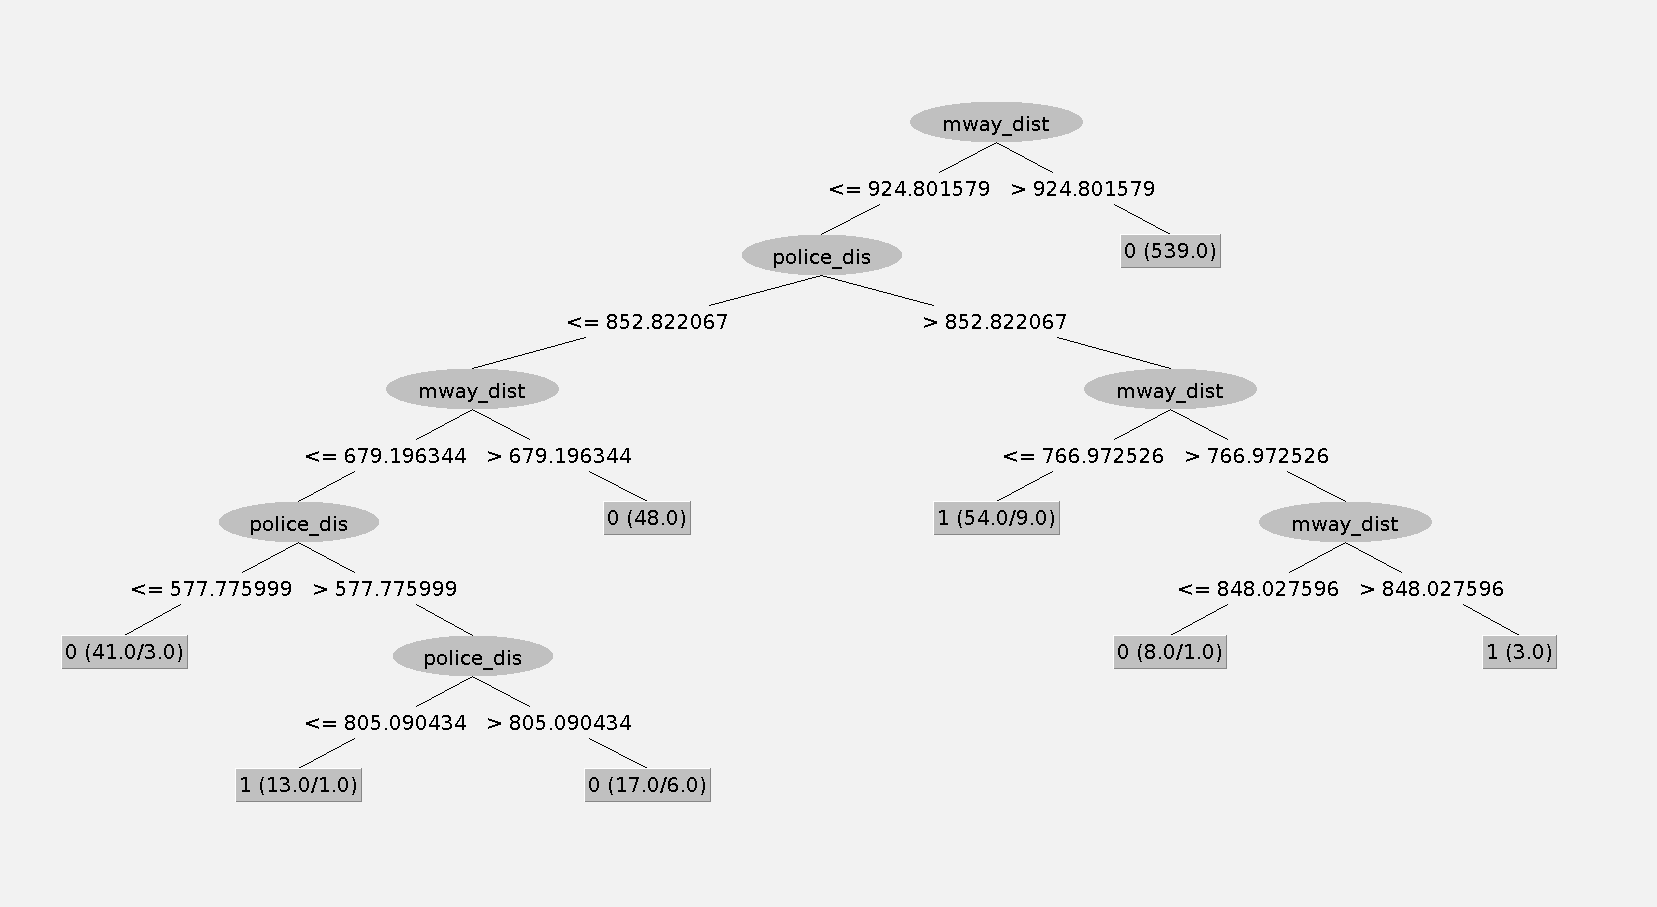
\includegraphics[width=\linewidth]{Decisiontree.png}
			\caption{J48 decision tree from weka}
			\label{dt}
		   \end{figure}
	
	    Extracted range include: -
\begin{table}[htbp]
	\centering
	\caption{Assignment of Linguistic Terms}
	\begin{tabular}{|l|l|}
		\hline
		\textbf{Motorway Distance Range} & \textbf{Linguistic Term} \\
		\hline
		0-679 & Very Low \\
		\hline
		0-766 & Low \\
		\hline
		766-848 & Medium-Low \\
		\hline
		766-924 & Medium \\
		\hline
		848-924 & Medium-High \\
		\hline
		679-924 & High-Medium \\
		\hline
		925 and above & High \\
		\hline
	\end{tabular}
	\label{tab:linguistic_terms}
\end{table}

\begin{table}[htbp]
	\centering
	\caption{Assignment of Linguistic Terms for Police Distance}
	\begin{tabular}{|l|l|}
		\hline
		\textbf{Police Distance Range} & \textbf{Linguistic Term} \\
		\hline
		0-577 & Very Low \\
		\hline
		577-805 & Low \\
		\hline
		577-852 & Medium-Low \\
		\hline
		805-852 & Medium High \\
		\hline
		852 and above & High \\
		\hline
	\end{tabular}
	\label{tab:linguistic_terms_police}
\end{table}

	
	
	\section{Rules}
	
	Attacked and not attacked rules are obtained from the figure \ref{dt} Decision tree based on the leaf nodes. 
	Example for the first rule which alone is capable of handling 539 atms from the dataset is given as \textgreater 924 in decision tree, which is converted to a \textbf{IF-THEN} rule for FIS as \textbf{IF} Motorway distance is greater than 924 \textbf{THEN} not attacked.\\    
	The following rules were obtained from the decision tree:-
	\begin{enumerate}
		\item IF \textbf{motorway distance} IS \textbf{high} THEN not attacked\\
		
		\item IF \textbf{motorway distance} IS \textbf{high-medium} AND \textbf{police distance} IS \textbf{medium-low} THEN not attacked\\
		
		\item IF \textbf{motorway distance} IS \textbf{very-low} AND \textbf{police distance} IS \textbf{very-low} THEN not attacked\\
		
		\item IF \textbf{motorway distance} IS \textbf{very-low} AND \textbf{police distance} IS \textbf{medium-high} THEN not attacked\\
		
		\item IF \textbf{motorway distance} IS \textbf{medium-low} AND \textbf{police distance} IS \textbf{high} THEN not attacked\\
		
		\item IF \textbf{motorway distance} IS \textbf{high-medium} AND \textbf{police distance} IS \textbf{very-low} THEN not attacked\\
		
		\item IF \textbf{motorway distance} IS \textbf{very-low} AND \textbf{police distance} IS \textbf{low} THEN attacked\\
		
		\item IF \textbf{motorway distance} IS \textbf{low} AND \textbf{police distance} IS \textbf{high} THEN attacked\\
		
		\item IF \textbf{motorway distance} IS \textbf{medium-high} AND \textbf{police distance} IS \textbf{high} THEN attacked\\
	\end{enumerate}


\section{Result}

\subsection{Control surface}
	\begin{figure}[h!]
	\centering
	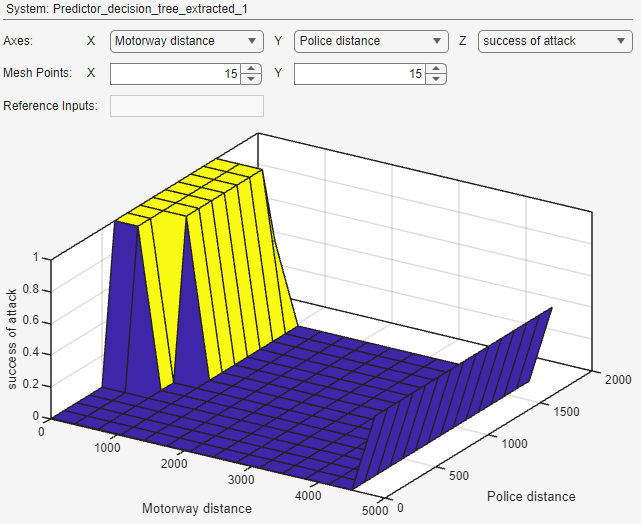
\includegraphics[width=\linewidth]{Fuzzy_final_control_surface.png}
	\caption{FIS control surface}
	\label{FISCS}
\end{figure}

In figure \ref{FISCS} The control surface shows us all the possible combination of inputs and the output associated with them.

The following observations can be made from the control surface: -
\begin{enumerate}
	\item Most of attack happens when distance is high from the police station and very low to medium from motorway distance.
	\item Attack is concentrated in a particular area indicating an attack pattern also visible in scatter plots. 
\end{enumerate} 

\subsection{Error distribution}

\begin{figure}[h!]
	\centering
	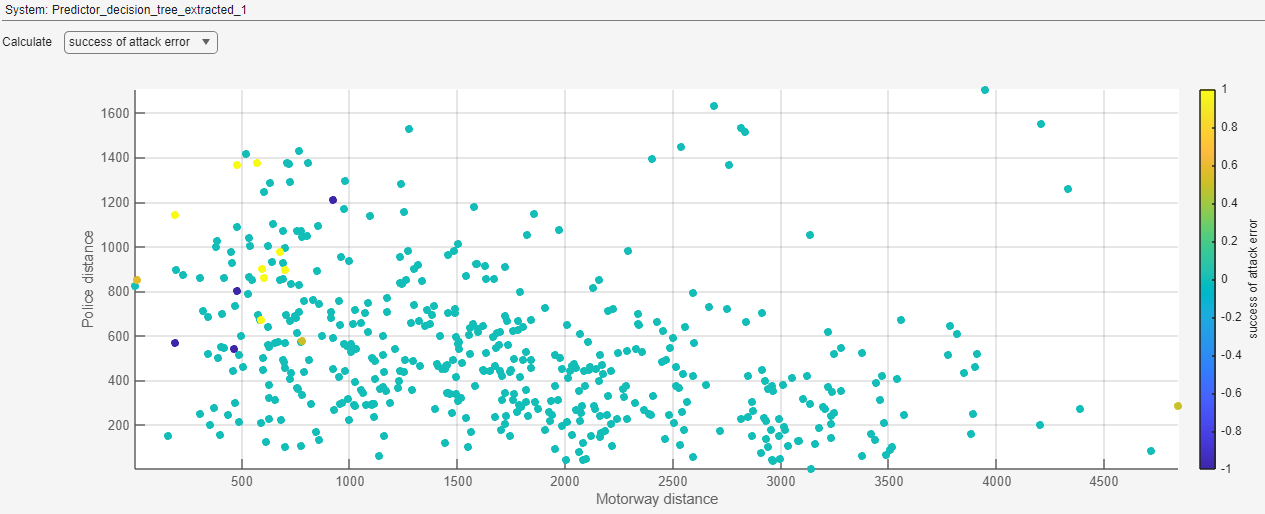
\includegraphics[width=\linewidth]{Fuzzy_final_error_distribution.png}
	\caption{FIS Error distribution}
	\label{FISED}
\end{figure}
    
    In figure \ref{FISED}, we can observe in which input range the attacked and not attacked atms classified are incorrect, based on this we can add further generic rules to minimize  the error rate.
    This helps in improving the accuracy and to have a look at internal workings of the model of the model which adds \textbf{room for further improvement} which is not possible with decision trees from weka or other machine learning models.
    
    \subsection{Model prediction}
    \begin{figure}[h!]
    	\centering
    	\includegraphics[width=\linewidth]{Fuzzy_final.png}
    	\caption{FIS Error distribution}
    	\label{FIS}
    \end{figure}
    
    In figure \ref{FIS} we can observe that the rules extracted from decision tree are working effectively in Fuzzy inference model and this FIS System validation can also help us to look at where exactly the decision tree is miss-classifying the output (Through error distribution).
    
    
    
    
 \section{Conclusion}
 From the above findings we can conclude that visualization can play a crucial role in understanding and handling the internals of predictive models. 
 
	Heuristic value is assigned to each rule in determining its significance for the overall prediction, The values are assigned based on inference from the leaf node with respect to correctly and incorrectly specified atms, but the robustnes of rules only allow minor up and down in the output even after changing the heuristic values significantly. Which signifies that rules are far more significant in handling the robustness of the model.
	
\section{Limitations}

Demographic variables were not included in this Fuzzy inference system because decision trees were not able to capture their predictive contribution with continuous value.\\ Decision trees were able to capture their predictive power with categorical values but using categorical value decreases the predictive performance of the model due to loss of information while converting the actual values to categorical values.

Due to less data on successfully attacked atms (only 70) the models(decision tree) learned to predict the not attacked atm(around 600) significantly better than predicting attacked atms which result s in less number of rules for attacked atms. This can be observed in continuous valued Figure \ref{dt} and the following categorical Figure.


 \begin{figure}[h!]
	\centering
	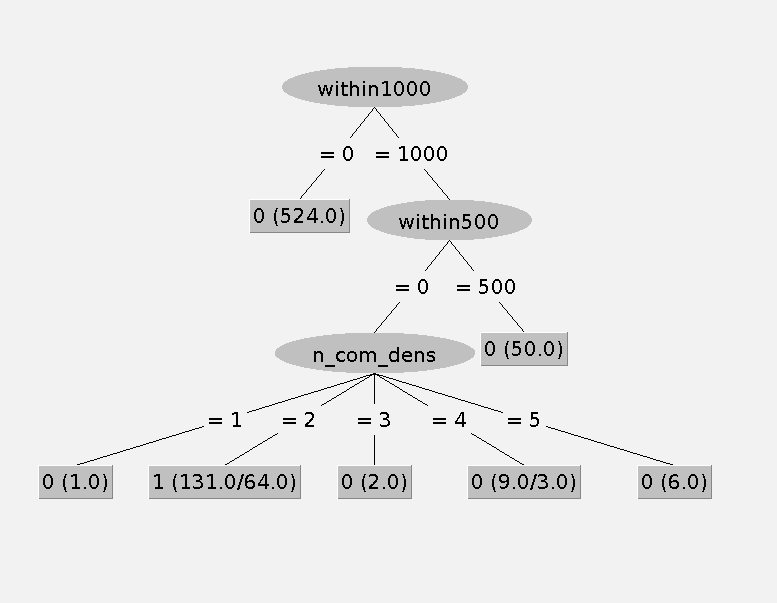
\includegraphics[width=\linewidth]{DTC.png}
	\caption{Decision Tree (categorical)}
	\label{DTC}
\end{figure}

	
	
	
	
	
	
	
	
	
	
	
\end{document}